\documentclass[12pt]{amsart}
\usepackage{style}

\author{Blake Farman}
\address{Lafayette College}
\title[Exam 2]{Exam 2\\Math 161}
\date{October 24, 2018}

\begin{document}
\maketitle

\begin{center}
  \fbox{\fbox{\parbox{5.5in}{\centering
        \noindent Answer the questions in the spaces provided on the
        question sheets and turn them in at the end of the exam period.\\


        \noindent It is advised, although not required, that you check your answers.
        All supporting work is required.
        Unsupported or otherwise mysterious answers will \textbf{not receive credit.}\\
        
        \noindent You may \textbf{not} use a calculator or any other electronic device, including cell phones, smart watches, etc.\\
        
        \noindent By writing your name on the line below, you indicate that you have read and understand these directions.}}}
\end{center}

\vspace{0.2in}
\makebox[\textwidth]{Name:\enspace\hrulefill}
\vspace{0.2in}

\theoremstyle{definition}
\newtheorem{thm}{}
\renewcommand{\qedsymbol}{}

\[
\begin{array}{|c|c|c|}
  \hline
  \text{Problem} & \text{Points Earned} & \text{Points Possible}\\
  \hline
  1 & & 5\\
  \hline
  2 & & 4\\
  \hline
  3 & & 2\\
  \hline
  4 & & 1\\
  \hline
  5 & & 3\\
  \hline
  6 & & 15\\
  \hline
  7 & & 20\\
  \hline
  8 & & 15\\
  \hline
  9 & & 15\\
  \hline
  10 & & 20\\
  \hline
  \text{Total} & & 100\\
  \hline
\end{array}
\]


\newpage
\section*{Fill In the Blank}
\begin{thm}[5 Points]
  Assume that $f$ is a function such that $f^\prime(x)$ and $f^{\prime\prime}(x)$ are defined for all $x$.
  \begin{enumerate}[(a)]
  \item
    A point \(c\) is a \textit{critical point} of \(f\) if \vspace{.15in}\\
    {\underline{\hspace{4in}}}.
    \vspace{.15in}
  \item
    $f$ is \textit{increasing} on an interval if {\underline{\hspace{1.5in}}} on that interval.
    \vspace{.15in}
  \item
    $f$ is \textit{decreasing} on an interval if {\underline{\hspace{1.5in}}} on that interval.
    \vspace{.15in}
  \item
    $f$ is \textit{concave up} on an interval if {\underline{\hspace{1.5in}}} on that interval.
    \vspace{.15in}
  \item
    $f$ is \textit{concave down} on an interval if {\underline{\hspace{1.5in}}} on that interval.
    \vspace{.15in}
  \end{enumerate}
\end{thm}

\begin{thm}[4 Points]
  The first derivative test says that a critical point, $c$, of $f$ is: \vspace{.15in}\\
  a \textit{local maximum} if $f^\prime$ changes from {\underline{\hspace{1.5in}}} to {\underline{\hspace{1.5in}}} at $c$;    \vspace{.15in}\\
  \textit{local minimum} if $f^\prime$ changes from {\underline{\hspace{1.5in}}} to {\underline{\hspace{1.5in}}} at $c$.
\end{thm}

\begin{thm}[2 Points]
  The second derivative test says that a critical point, $c$, of $f$ is:\vspace{.15in}\\
  a \textit{local maximum} if $f^{\prime\prime}$ is {\underline{\hspace{1.5in}}} at $c$;\vspace{.15in}\\
  a \textit{local minimum} if $f^{\prime\prime}$ is {\underline{\hspace{1.5in}}} at $c$.
  \vspace{.15in}
\end{thm}
\begin{thm}[1 Point]
  Suppose that $f^{\prime\prime}(c)=0$.  We say $c$ is an inflection point of $f$ if\vspace{.15in}\\
  {\underline{\hspace{4in}}}.
\end{thm}

\begin{thm}[Mean Value Theorem - 3 Points]
  Let $f$ be a function satisfying
  \vspace{.15in}
  \begin{enumerate}[1.]
  \item
    $f$ is {\underline{\hspace{1.5in}}} on $[a,b]$, and
    \vspace{.15in}
  \item
    $f$ is {\underline{\hspace{1.5in}}} on $(a,b)$.
  \end{enumerate}
  \vspace{.15in}
  Then there exists a $c$ in $(a,b)$ such that
  \[f^\prime(c)={\underline{\hspace{1.5in}}}\].
\end{thm}

\newpage

\section*{Problems}

\begin{thm}[15 Points]
  Find $dy/dx$: $$\cos(xy)=1+\tan y$$
\end{thm}

\vspace{3in}

\begin{thm}[20 Points]
  A street light is mounted at the top of a 15-ft-tall pole.  A person 6 ft tall walks away from the pole with a speed of 5 ft/s along a straight path.  How fast is the tip of their shadow moving when they are 40 ft from the pole?\\ (Hint: The length of the shadow is measured from the person to the tip of the shadow; the rate at which the tip of the shadow is moving is measured from the pole to the tip of the shadow.)
\end{thm}

\newpage

\begin{thm}[15 Points]
  Find the value or values of $c$ that satisfy the conclusion of the Mean Value Theorem for the function $f(x)=x^3 - 2x^2 -4x + 2$ on $[-2,2]$.
\end{thm}

\vspace{3in}

\begin{thm}[15 Points]
  Find the absolute maximum and minimum values of $f(x)=2x^3 - 3x^2 -12x + 1$ on $[-2,3]$.
\end{thm}

\newpage

\begin{thm}[20 Points]
  Sketch the curve $$f(x)=\frac{x^2}{x-1}$$
  \begin{enumerate}[(a)]
  \item\label{sketching first step}
    State the domain of \(f\).
    \vspace{1in}
    
  \item
    Find the intercepts and express them as an \((x,y)\) pair.
    Write NONE if there are none.\\ \\
    x-intercepts:\hskip .5 truein \hrulefill\\ \\
    y-intercept:\hskip .5 truein \hrulefill
    \vspace{1in}
  \item
    Is the function even, odd, or neither? What type of symmetry does the function have?
    \vspace{1in}
  \item
    Find the asymptotes.
    Write NONE if there are none.\\ \\
    Horizontal:\hskip .5 truein \hrulefill\\ \\
    Oblique:\hskip .5 truein \hrulefill\\\ \\
    Vertical:\hskip .5 truein \hrulefill
    \newpage
  \item
    Find the intervals where the function is increasing and decreasing.
    Write NONE if not applicable.\\ \\
    Increasing:\hskip .5 truein \hrulefill\\ \\
    Decreasing:\hskip .5 truein \hrulefill
    \vspace{3in}
  \item
    State the local maximum and local minimum value(s).
    Write NONE if not applicable.\\ \\
    Local maximum value(s):\hskip .5 truein \hrulefill\\ \\
    Local minimum value(s):\hskip .5 truein \hrulefill
    \newpage
  \item\label{sketching penultimate step}
    Find the intervals on which the function is concave up and concave down. State the inflection points.
    Write NONE if not applicable.\\ \\
    Concave Up:\hskip .5 truein \hrulefill\\ \\
    Concave Down:\hskip .5 truein \hrulefill\\ \\
    Inflection Points:\hskip .5 truein \hrulefill
    \vspace{2in}
  \item
    Use your answers to Parts~\eqref{sketching first step}-\eqref{sketching penultimate step} to sketch the curve.
    Be sure that your graph is labeled and neat. Messy/incoherent graphs will receive zero points.
    \begin{center}
      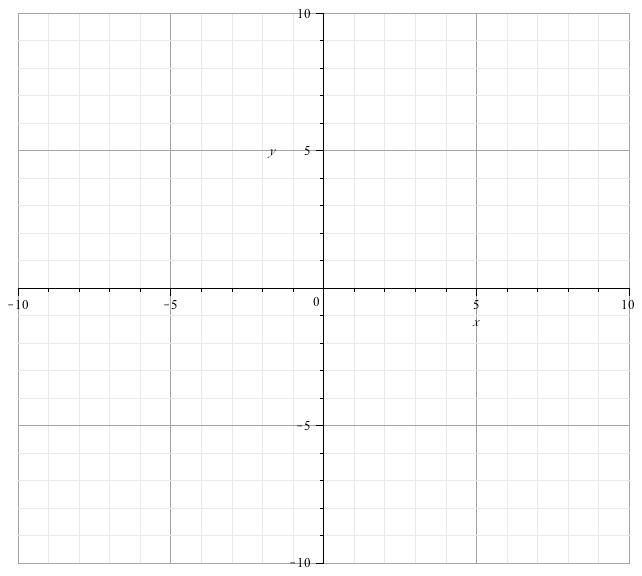
\includegraphics[scale=0.5]{graphpaper.jpg}
    \end{center}
  \end{enumerate}
\end{thm}
\end{document}
